% -*- root: ../main.tex -*-
\chapter{Consenso e State Machine Replication}
Il principale vantaggio fornito dai sistemi distribuiti rispetto ai sistemi centralizzati sta nel fatto di poter garantire un servizio continuo malgrado \textit{failures} e \textit{malfunzionamenti} \cite[Friedman:1996]{Friedman:1996}.
L'idea infatti è quella di poter realizzare sistemi che possano far fonte a componenti inaffidabili che non possono garantire una disponibilità costante; questi sistemi devono essere in grado di \textit{reagire} e \textit{adattarsi} automaticamente ai cambiamenti.\\
Fra le sfide più importanti che i sistemi distribuiti devono affrontare al giorno d'oggi troviamo: la gestione delle failures, la coordinazione, il discovery di servizi e la gestione della configurazione; tutti problemi difficili da risolvere in ambienti dinamici. Fortunatamente il consenso distribuito permette di risolvere gran parte di questi problemi.
	
	\section{Il problema del Consenso}
	Gli algoritmi di consenso rappresentano gli algoritmi fondamentali e più importanti nell'ambito dei sistemi distribuiti.
	Gli algoritmi di consenso permettono a una collezione di \textbf{macchine eterogenee} di lavorare in qualche modo come se fossero un \textbf{una sola macchina}.\\
	Si parte dunque con un insieme di \textbf{macchine} singolarmente \textbf{inaffidabili} e si fa in modo che esse si comportino come un'\textbf{unica macchina super-affidabile} che garantisce di operare in modo reliable anche nel caso in cui alcune macchine falliscano.\\
	All'interno di un gruppo di consenso (\textbf{consensus group}) i fallimenti sono gestiti in un modo studiato e comprovato, questo permette di avere un \textit{modello di funzionamento} robusto e affidabile.\\
	Data l'estremam \textbf{availability} e \textbf{raliability} dei consensus group, altri sistemi possono decidere di usare un consensus group come fondamenta per garantire fault tolerance; questo porta gli algoritmi di consenso a giocano un ruolo fondamentale nella costruzione di sistemi reliable di grandi dimensioni. 

	\section{Replicated State Machine}
	Gli algoritmi di consenso sono generalmente utilizzati nel contesto di quelle che chiamiamo replicated state machines. Prima di parlare di macchine a stati replicate bisogna definire cos'è una macchina a stati.\\
	Una macchina a stati è generalmente un programma che: 
	\begin{itemize}
		\item{\textit{accetta e risponde} a vari tipi di interazioni o \textbf{stimoli esterni}.}
		\item{Gli stimoli possono essere nella forma di \textit{comandi} che provengono da clients e hanno lo scopo di gestire lo \textbf{stato interno} della macchina.}
	\end{itemize}
	Al giorno d'oggi le state machine rappresentano un modello generale di computazione estremamente diffuso. Gran parte dei sistemi a larga scala (as-a-service) che utilizziamo solitamente sono nella forma di macchine a stati.

	\begin{figure}[H]
		\centering
		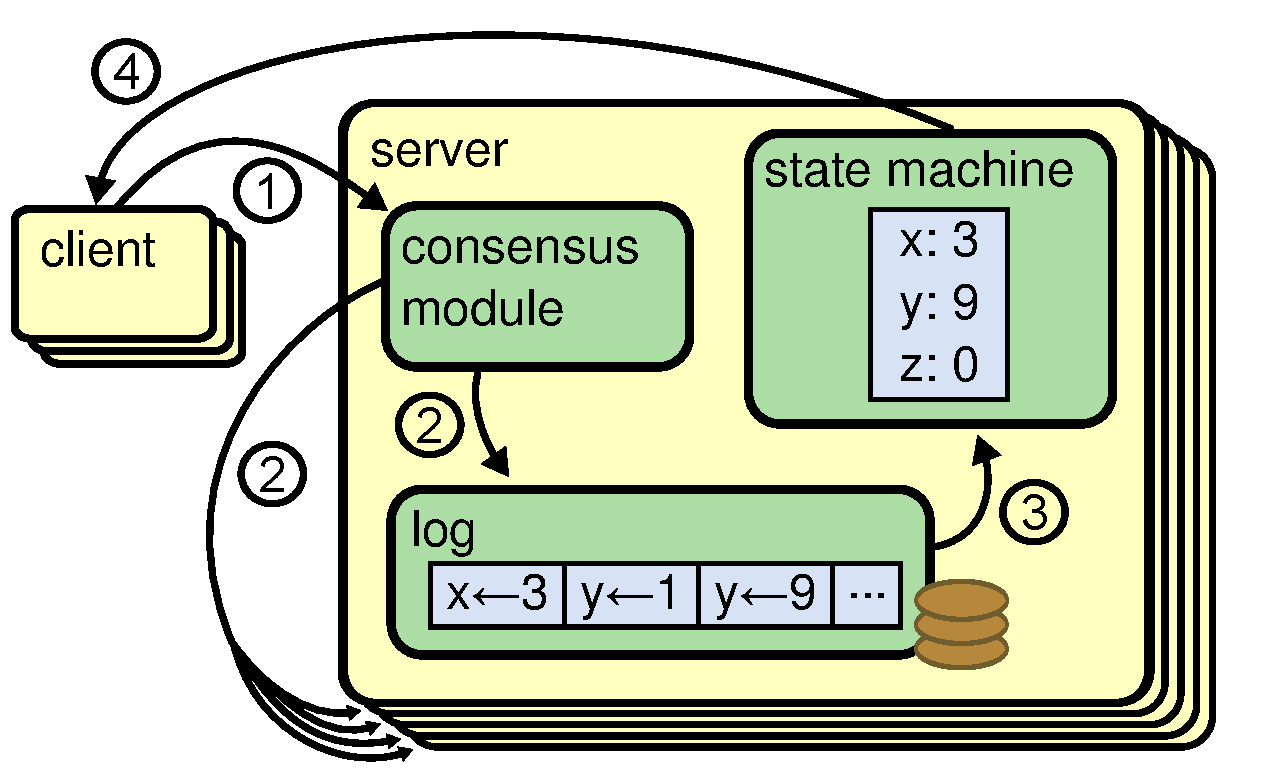
\includegraphics[width=0.99\columnwidth]{statemachine}
		\caption{Un modello di state machine semplificato}
		\label{fig:figure1}
	\end{figure}  